%!TEX root = prelim.tex
%!TEX root = fakeroot.tex
\subsection{Contiguous Occlusion}

\renewcommand{\imagesizestring}{height}
\renewcommand{\imagesizea}{0.25\textheight}
\renewcommand{\imagesizeb}{0.15\textheight}


\frame{\frametitle{SRC on Random Corruption}
\renewcommand{\imagesizestring}{height}
\renewcommand{\imagesizea}{0.10\textheight}
\vspace{-.1in}
\begin{itemize}
\item<1-> SRC is provably optimal for {\em randomized} corruption. 
\begin{center}
\begin{columns}
\begin{column}{0.5\textwidth}
%{\footnotesize Yale Dataset, 19 images per person:}
\begin{center}
\begin{tabular}{@{}cccc@{}}
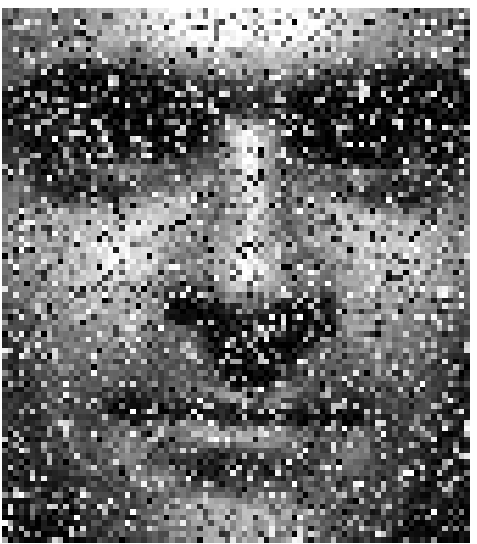
\includegraphics[\imagesizestring=\imagesizea]{IEEEPAMI_Occlusion/figures/ysp-30-125-o.pdf} &
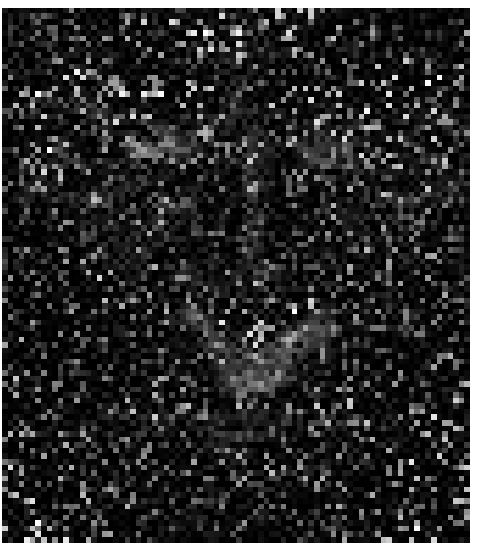
\includegraphics[\imagesizestring=\imagesizea]{IEEEPAMI_Occlusion/figures/ysp-30-125-e.pdf} &
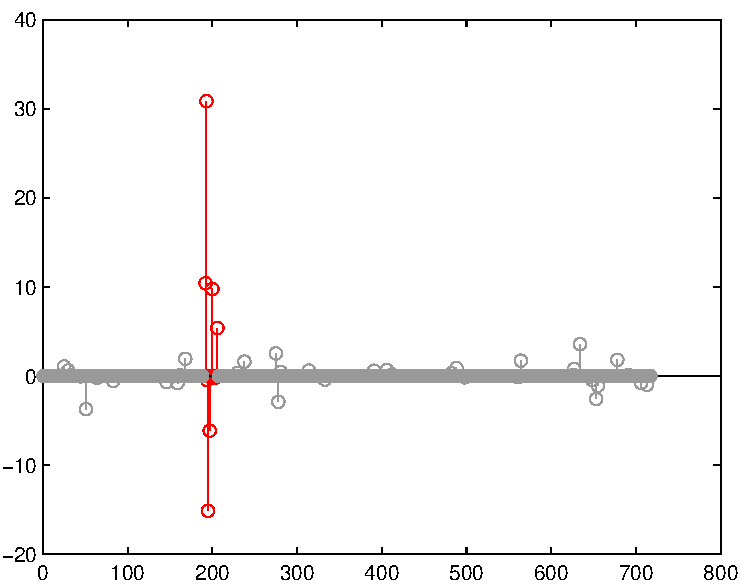
\includegraphics[\imagesizestring=\imagesizea]{IEEEPAMI_Occlusion/figures/ysp-30-125-w.pdf} &
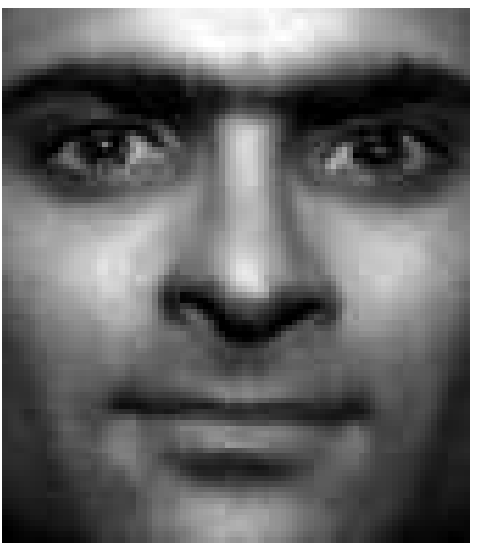
\includegraphics[\imagesizestring=\imagesizea]{IEEEPAMI_Occlusion/figures/ysp-30-125-r.pdf} \\[-.05in]
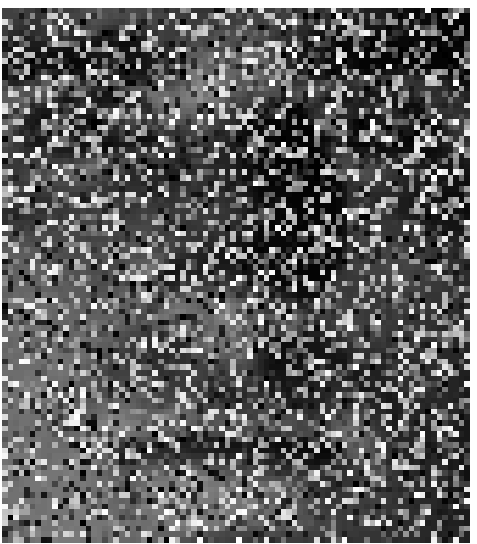
\includegraphics[\imagesizestring=\imagesizea]{IEEEPAMI_Occlusion/figures/ysp-50-379-o.pdf} &
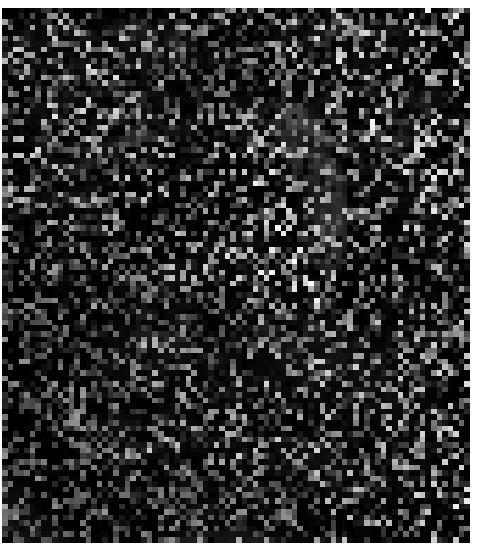
\includegraphics[\imagesizestring=\imagesizea]{IEEEPAMI_Occlusion/figures/ysp-50-379-e.pdf} &
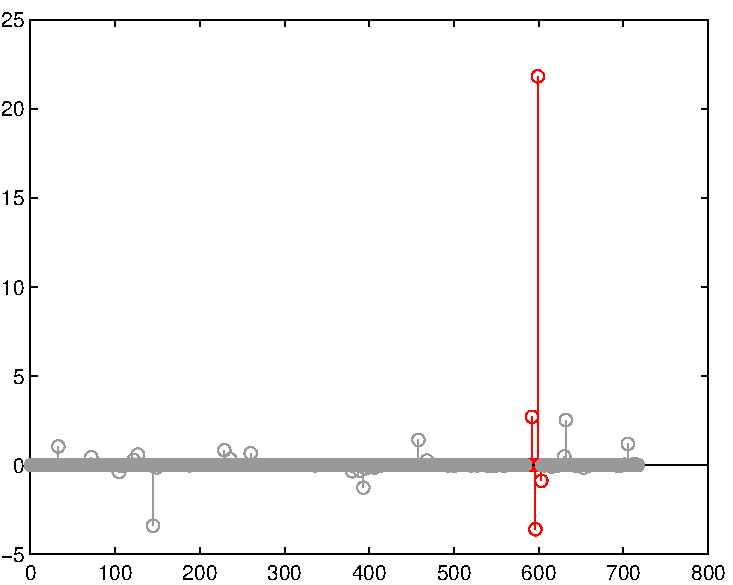
\includegraphics[\imagesizestring=\imagesizea]{IEEEPAMI_Occlusion/figures/ysp-50-379-w.pdf} &
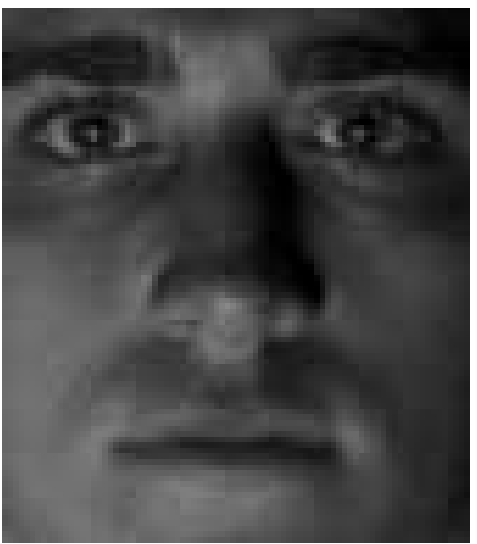
\includegraphics[\imagesizestring=\imagesizea]{IEEEPAMI_Occlusion/figures/ysp-50-379-r.pdf} \\[-.05in]
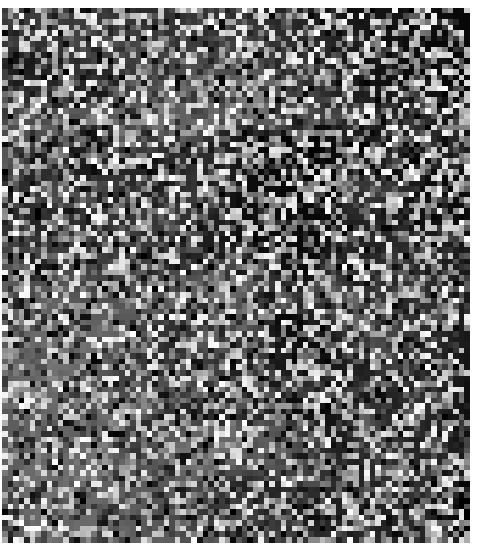
\includegraphics[\imagesizestring=\imagesizea]{IEEEPAMI_Occlusion/figures/ysp-70-80-o.pdf} &
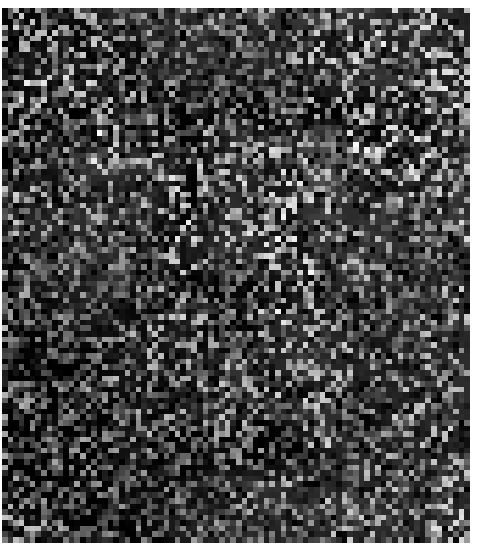
\includegraphics[\imagesizestring=\imagesizea]{IEEEPAMI_Occlusion/figures/ysp-70-80-e.pdf} &
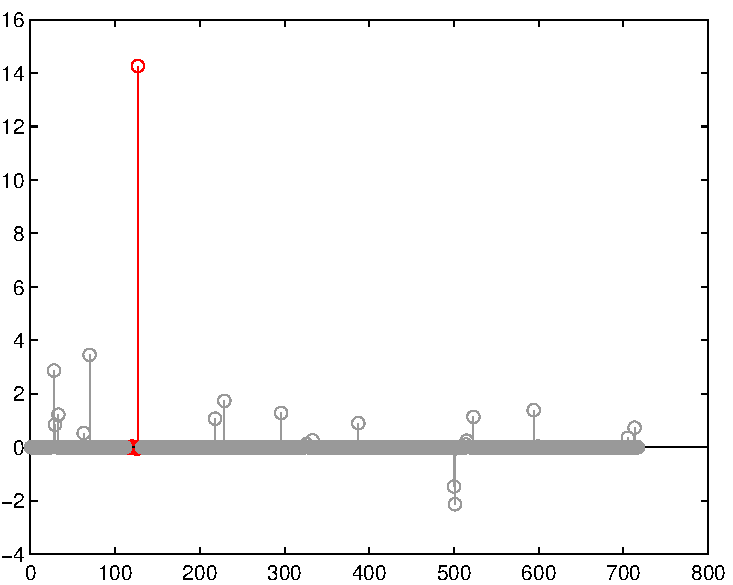
\includegraphics[\imagesizestring=\imagesizea]{IEEEPAMI_Occlusion/figures/ysp-70-80-w.pdf} &
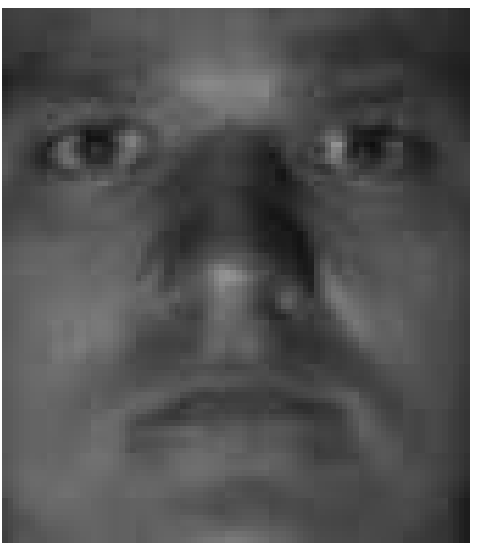
\includegraphics[\imagesizestring=\imagesizea]{IEEEPAMI_Occlusion/figures/ysp-70-80-r.pdf}\\[-.1in]
{\tiny Test Image} & {\tiny Error} & {\tiny Coefficients} & {\tiny Reconstruction}
\end{tabular}
\end{center}
\end{column}
\begin{column}{0.5\textwidth}
\begin{center}
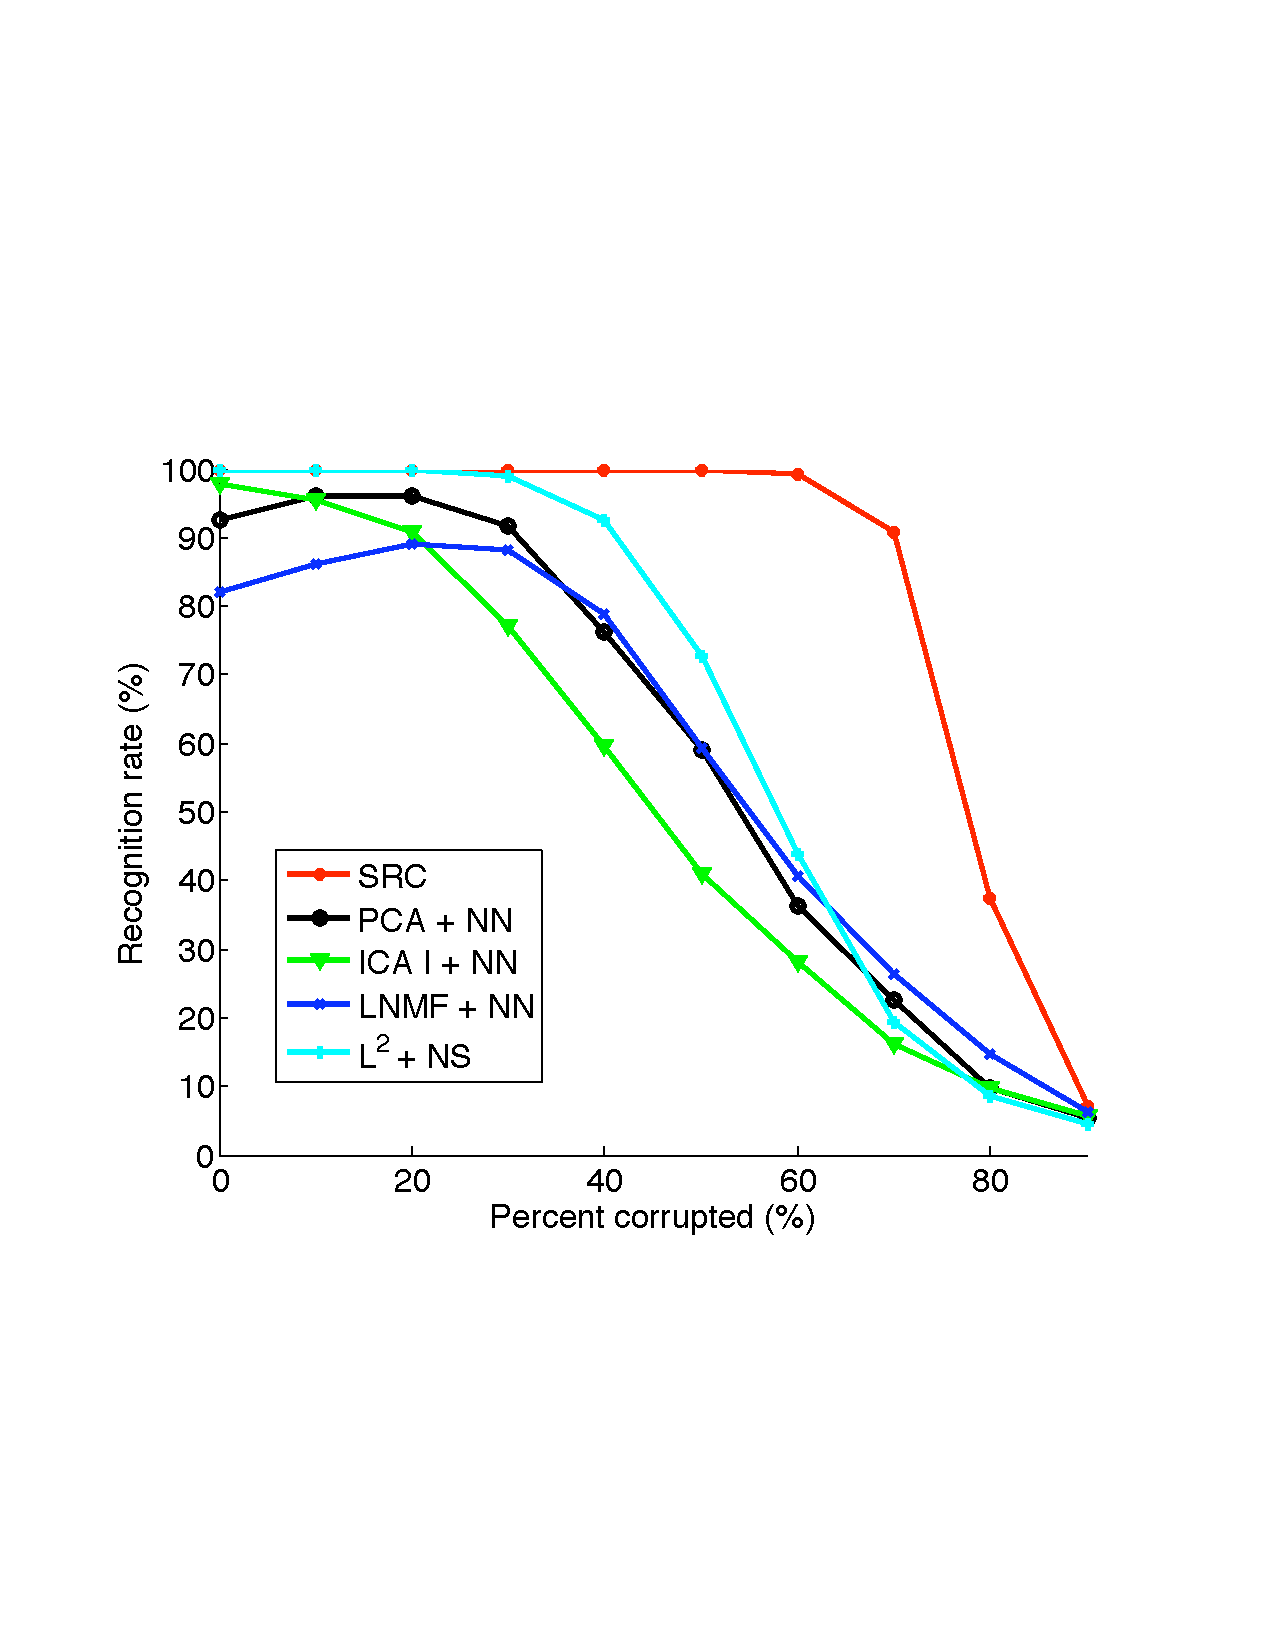
\includegraphics[height=.3\textheight]{IEEEPAMI_Occlusion/figures/yb_result_rc.pdf}\\
\end{center}
\end{column}
\end{columns}

\end{center}
%\vspace{.3in}
\item<2-> For contiguous occlusion, SRC can handle up to 30\% occlusion.\\
\begin{columns}
\begin{column}{0.5\textwidth}
\begin{center}
\begin{tabular}{@{}cccc@{}}
\includegraphics[\imagesizestring=\imagesizea]{IEEEPAMI_Occlusion/figures/352-30-o.pdf} &
\includegraphics[\imagesizestring=\imagesizea]{IEEEPAMI_Occlusion/figures/352-30-e.pdf}&
\includegraphics[\imagesizestring=\imagesizea]{IEEEPAMI_Occlusion/figures/352-30-w.pdf}&
\includegraphics[\imagesizestring=\imagesizea]{IEEEPAMI_Occlusion/figures/352-30-r.pdf} \\[-.05in]
\includegraphics[\imagesizestring=\imagesizea]{IEEEPAMI_Occlusion/figures/395-30-o.pdf} &
\includegraphics[\imagesizestring=\imagesizea]{IEEEPAMI_Occlusion/figures/395-30-e.pdf}&
\includegraphics[\imagesizestring=\imagesizea]{IEEEPAMI_Occlusion/figures/395-30-w.pdf} &
\includegraphics[\imagesizestring=\imagesizea]{IEEEPAMI_Occlusion/figures/395-30-r.pdf}\\[-.05in]
{\tiny Test Image} & {\tiny Error} & {\tiny Coefficients} & {\tiny Reconstruction}
\end{tabular}
\end{center}
\end{column}
\begin{column}{0.5\textwidth}
\begin{center}
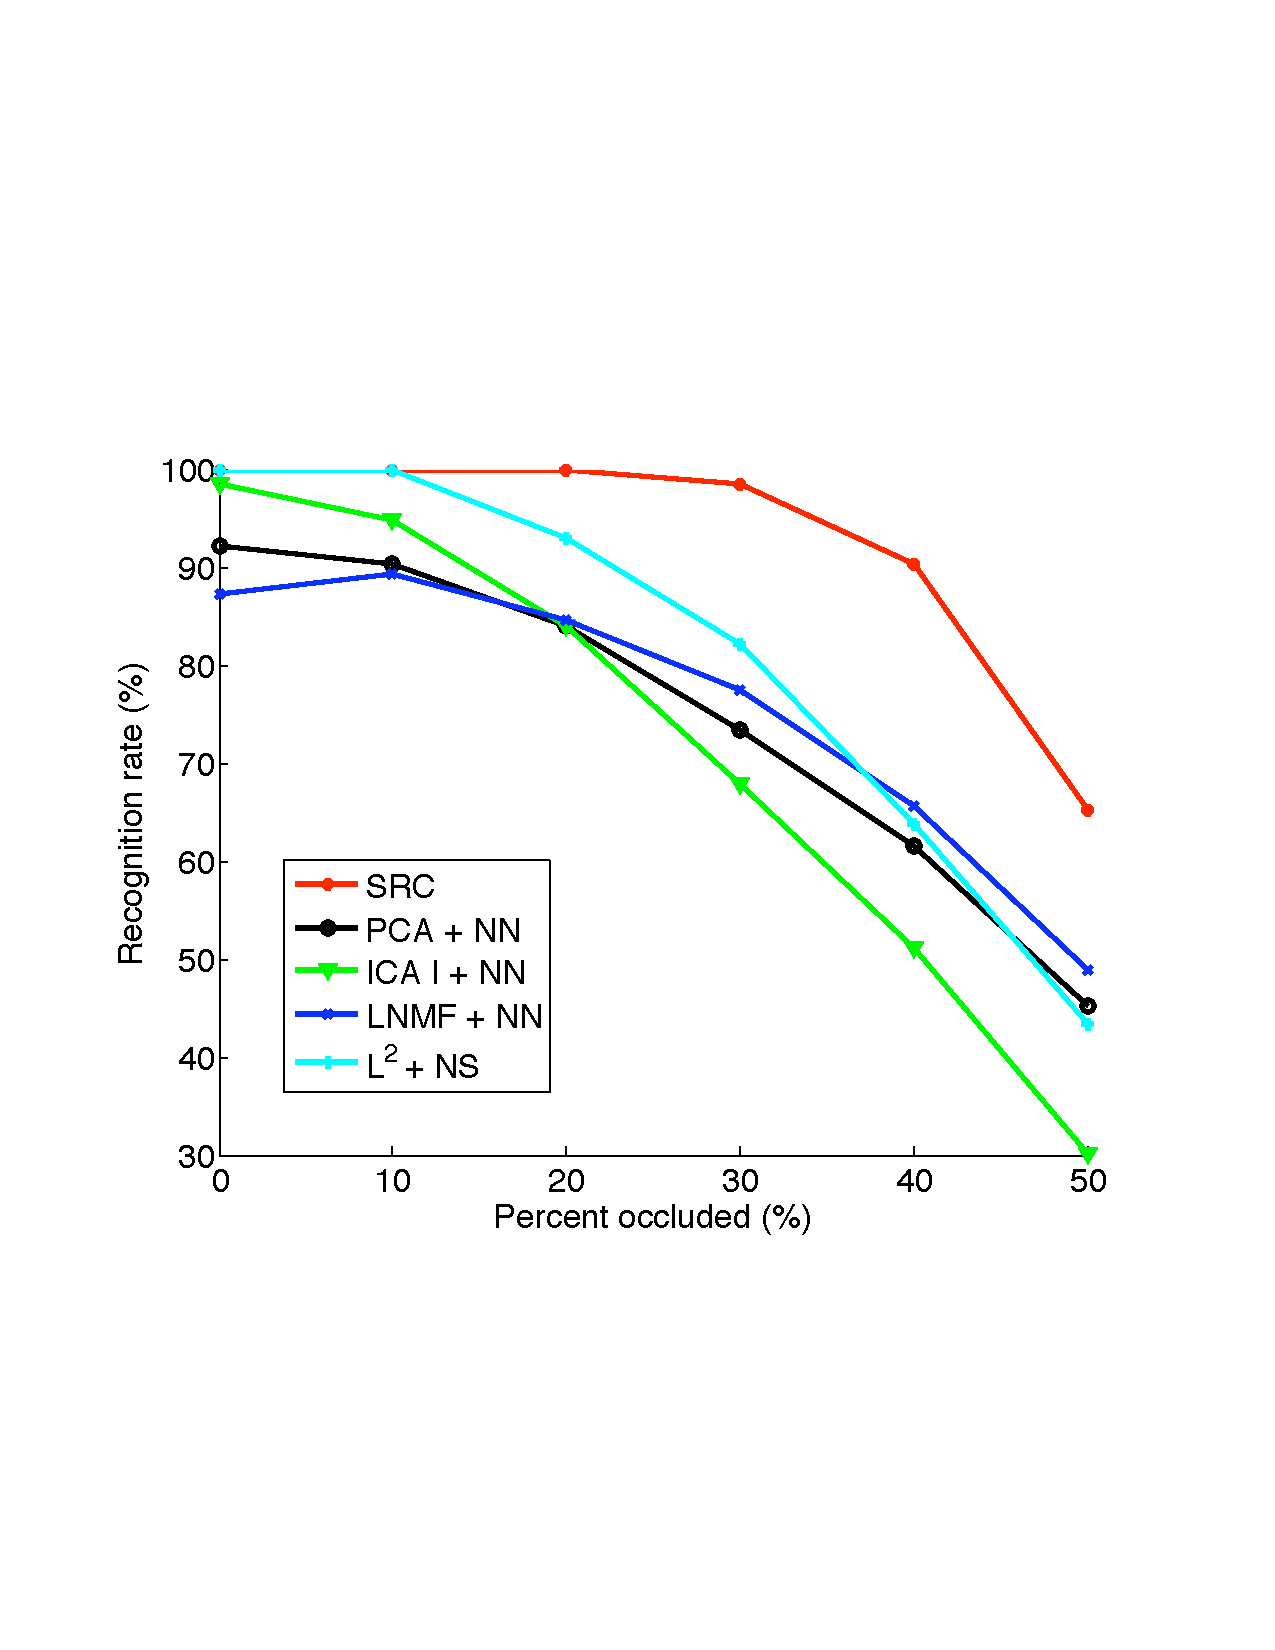
\includegraphics[height=.3\textheight]{IEEEPAMI_Occlusion/figures/yb_result_bab.pdf}
\end{center}
\end{column}
\end{columns}
\item<2-> Can we do better for spatially contiguous occlusions?
\end{itemize}
}




%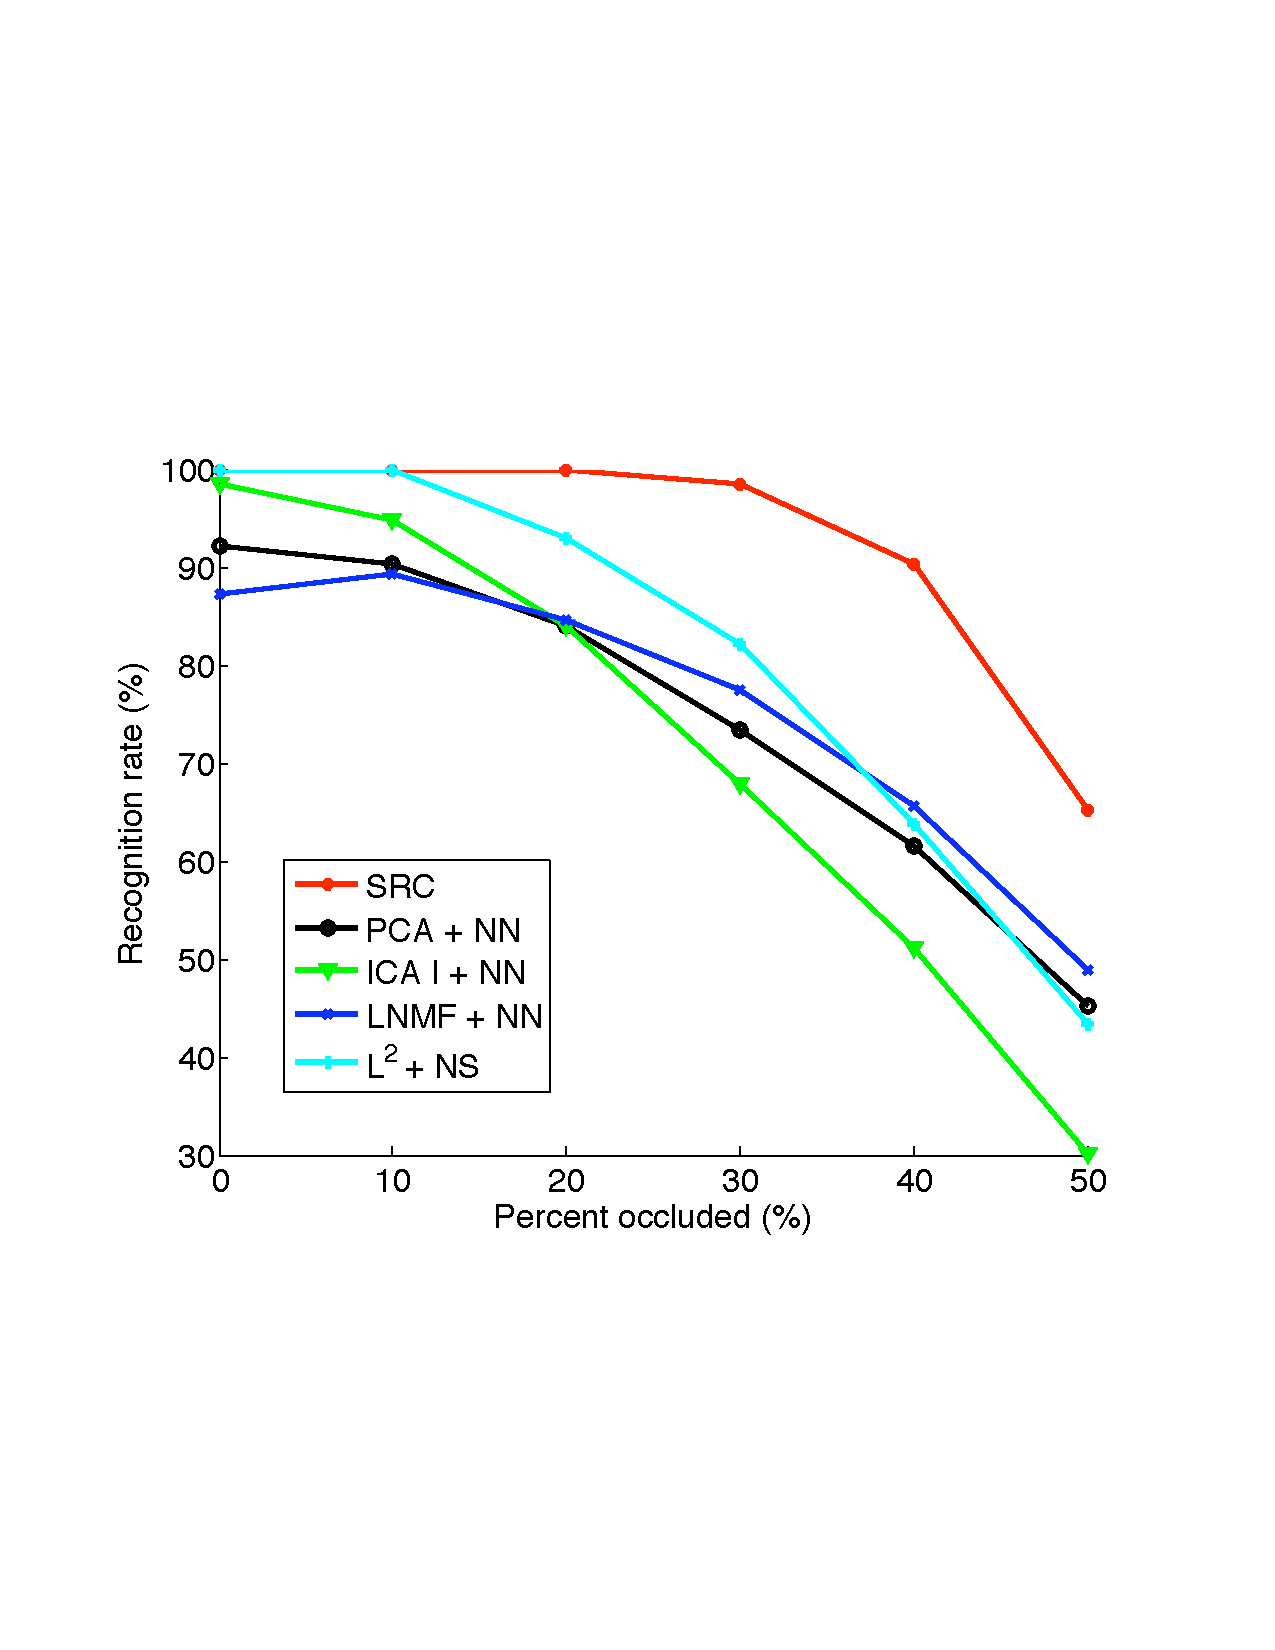
\includegraphics[width=2.9in]{IEEEPAMI_Occlusion/figures/yb_result_bab.pdf}




\frame{\frametitle{Markov Random Field Model}
\vspace{-.1in}
\begin{center}

\includegraphics[width=.35\textwidth]{images/lattice.pdf}\\
\vspace{-.15in}{\tiny Markov Random Field (MRF)}
\end{center}
\vspace{-.1in}
\begin{itemize}
\item Represent the image domain as an adjacency graph $G=(V,E)$
\item Let $\s\in \{-1,1\}^m$ be the support of $\e[i]$ :\\  $\s[i] = \left\{\begin{array}{cl} -1 & \mbox{for } \e[i] = 0\\ 1 & \mbox{for } \e[i] \neq 0 \end{array}\right.$
\item Model probability mass function of $\s$ using classical Ising model:
\begin{equation*}
p(\s) \propto \exp\Bigl\{\underbrace{\sum_{(i,j)\in E}\lambda_{ij}\s[i]\s[j]}_{\tiny \mbox{edge prior}} + \underbrace{\sum_{i\in V}\lambda_i \s[i]}_{\tiny \mbox{vertex prior}}\Bigr\}
\end{equation*}
\end{itemize}
}

\frame{\frametitle{Applying MRF to Occlusion}
\vspace{-.1in}
\begin{itemize}
\item Use simplified Ising Model: $p(\s) \propto \exp\Bigl\{\sum_{(i,j)\in E}\lambda \s[i]\s[j] \Bigr\}$
\item joint p.d.f of $\e$: \\ 
\vspace{-.15in}
\begin{eqnarray*}
p(\e,\s) &=& p(\s) p(\e|\s) = p(\s) \prod_i p(\e[i]|\s[i])\\  
&\propto&  \exp\Big\{\hspace{-0mm}\sum_{(i,j)\in E} \hspace{-0mm}\lambda\s[i]\s[j] + \sum_{i\in V} \log p(\e[i] \mid \s[i]) \Big\}
\end{eqnarray*}
\item approximate p($\e|\s$):\\
\begin{center}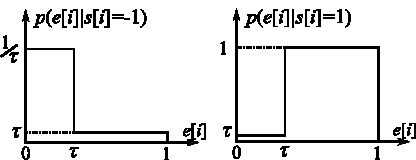
\includegraphics[width=0.5\textwidth]{figures_iccv/function.pdf}\end{center}
\end{itemize}
}

%\item Isolate effect of occlusion by assuming aligned images

%
%\frame{\frametitle{Solving Sparse Representation under MRF assumption}
%\begin{itemize}
%\item Want to solve 
%$\hat \s = \mbox{arg}\max_{\x_k,\e,\s} p(\s, \e) \quad \mbox{s.t.} \quad \y = A_k \x_k + \e.$
%\item Difficult non-convex optimization problem!
%\item $\Rightarrow$ alternate between: \begin{enumerate} 
%\item Performing sparse representation using pixels labeled as un-occluded: \\
%\begin{equation*}(\hat{\x}_k,\hat{\e}^*) = \argmin{\x,\e^*} \|\e^*\|_1  \; \textup{ s.t. } \; \y^* = A_k^*\x+\e^*, \x\geq 0 \end{equation*}
%\item Estimating the support of the occlusion given the representation error: \\
%\begin{equation*} \hat{\s} = \argmax{\s \in \{-1,1\}^m}  \sum_{(i,j)\in E}  \lambda \s[i]\s[j] + \sum_{i\in V} \log p(\e[i] | \s[i]).\end{equation*}
%\end{enumerate}
%\end{itemize}
%}

\frame{\frametitle{Solving Sparse Representation under MRF assumption}
\begin{itemize}
\item Want to solve 
$\hat \s = \mbox{arg}\max_{\x_k,\e,\s} p(\s, \e) \quad \mbox{s.t.} \quad \y = A_k \x_k + \e.$
\item Difficult non-convex optimization problem!
\item $\Rightarrow$ alternate between: \begin{enumerate} 
\item Solving $(\hat \x_k, \hat \e) = \mbox{arg}\max_{\x_k,\e} p(\s, \e) \quad \mbox{s.t.} \quad \y = A_k \x_k + \e.$\\
	 For very small $\tau$, this reduces (approximately) to solving SRC on a restricted domain:
	\begin{equation*}(\hat{\x}_k,\hat{\e}^*) = \argmin{\x,\e^*} \|\e^*\|_1  \; \textup{ s.t. } \; \y^* = A_k^*\x+\e^*, \x\geq 0 \end{equation*}
\item Solving $\hat \s = \mbox{arg}\max_{\s} p(\s, \e) \quad \mbox{s.t.} \quad \y = A_k \x_k + \e.$\\
	Under our assumptions this reduces to:
	\begin{equation*} \hat{\s} = \argmax{\s \in \{-1,1\}^m}  \sum_{(i,j)\in E}  \lambda \s[i]\s[j] + \sum_{i\in V} \log p(\e[i] | \s[i]).\end{equation*}
\end{enumerate}
\end{itemize}
}


\frame{\frametitle{The Complete MRF Recognition Algorithm}
{\footnotesize
\begin{algorithmic}[1]
\STATE {\bf Input:} A matrix of normalized training samples $A =
[A_1,A_2,\ldots,A_K] \in \Re^{m\times n}$ for $K$ classes, a test
sample $\y \in \Re^{m}$.

\FOR{each subject $k$}

\STATE Initialize the error support $\s^{(0)}_k = \mathbf{-1}_m$.

\STATE {\bf repeat}

\STATE \hspace{3mm}$A_k^* = A_k[\s^{(t-1)}_k=-1,\, :\, ]$, $\y^* =
\y[s^{(t-1)}_k=-1]$;

\STATE \hspace{3mm}Solve the convex program\\
\hspace{5mm} $(\hat{\x}_k,\hat{\e}^*) \;=\; \arg\min \|\e^*\|_1 $\\
\hspace{24mm} $\mathrm{ s.t. } \quad \y^* = A_k^*\x+\e^*, \, \x\geq 0;$

\STATE \hspace{3mm}$\hat{\e}_k\leftarrow \y-A_k\hat{\x}_k$;

\STATE \hspace{3mm}Update error support via graph cuts:\vspace{0mm}
$$\s^{(t)}_k = \arg\hspace{-4mm}\max_{\s\in\{-1,1\}^m}\hspace{-2mm}\sum_{i,j\in
E}\hspace{-2mm}{\lambda} \s[i]\s[j]+\sum_{i\in
V}\log\big(p(\hat{\e}_k[i]|\s[i])\big);$$\vspace{0mm}
\STATE {\bf until} maximum iterations or convergence.

\STATE Compute the normalized error $$\mathbf{r}_k(\y) =
\frac{\|\y^*-A_k^*\hat{\x}_k\|_1}{|\{ i \mid \s_k[i] = -1 \}|^2}. \vspace{0mm}$$
\ENDFOR

\STATE {\bf Output:} identity$(\y) = \arg\min_k \r_k(\y)$.
\end{algorithmic}
}}

\subsection{Experiments}

\frame{\frametitle{Choosing Model Parameters}
\begin{itemize}
\item Meaning of $\tau$ and $\lambda$: \begin{itemize}\item larger $\lambda$ smoothes $\s$ at the expense of increasing $\e$. \item $\tau$ is a threshold on $\e$, above which pixel is considered occluded \end{itemize}
\item For a given $\lambda$, the support of $\e$ will drop off suddenly as $\tau$ is decreased:
\begin{center}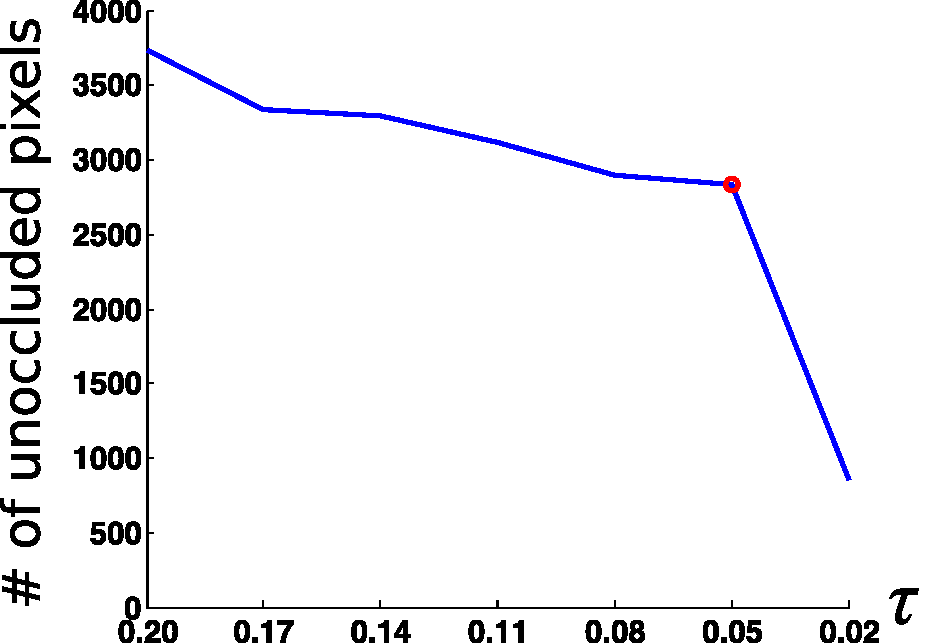
\includegraphics[width=0.5\textwidth]{figures_iccv/n_of_goodentry.pdf}\end{center}
\item{Beyond red point many unoccluded pixels get mis-labelled as occluded.}
\end{itemize}
}


\renewcommand{\imagesizestring}{height}
\renewcommand{\imagesizea}{0.15\textheight}
\frame{\frametitle{Effect of $\tau$ and $\lambda$}
Example test image from AR database, occluded by scarf: \\
\begin{center}
\fbox{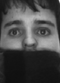
\includegraphics[height=0.225\textheight]{figures_iccv/test_epsilon.png}}\\
\end{center}
Error support for varying $\lambda, \tau$:
\begin{tabular}{cccccccb{.120\textwidth}}
$\lambda = 1$ &
\fbox{
\includegraphics[height=\imagesizea]{figures_iccv/epsilon1/20.png}}&
\fbox{
\includegraphics[height=\imagesizea]{figures_iccv/epsilon1/17.png}}&
\fbox{
\includegraphics[height=\imagesizea]{figures_iccv/epsilon1/14.png}}&
\fbox{
\includegraphics[height=\imagesizea]{figures_iccv/epsilon1/11.png}}&
\fbox{
\includegraphics[height=\imagesizea]{figures_iccv/epsilon1/8.png}}&
\fbox{
\includegraphics[height=\imagesizea]{figures_iccv/epsilon1/5.png}}&
\fbox{
\includegraphics[height=\imagesizea]{figures_iccv/epsilon1/2.png}}\\
$\lambda = 3$&
\fbox{
\includegraphics[height=\imagesizea]{figures_iccv/epsilon3/20.png}}&
\fbox{
\includegraphics[height=\imagesizea]{figures_iccv/epsilon3/17.png}}&
\fbox{
\includegraphics[height=\imagesizea]{figures_iccv/epsilon3/14.png}}&
\fbox{
\includegraphics[height=\imagesizea]{figures_iccv/epsilon3/11.png}}&
\fbox{
\includegraphics[height=\imagesizea]{figures_iccv/epsilon3/8.png}}&
\fbox{
\includegraphics[height=\imagesizea]{figures_iccv/epsilon3/5.png}}&
\fbox{
\includegraphics[height=\imagesizea]{figures_iccv/epsilon3/2.png}}\\
 &$\tau=0.2$ & 0.17 & 0.14 & 0.11 & 0.08 & 0.05 & 0.02
\end{tabular}
}

\renewcommand{\imagesizestring}{width}
\renewcommand{\imagesizea}{0.2\textwidth}
\frame{\frametitle{Example Recovery from Synthetic Occlusion}
\begin{columns}
\begin{column}{0.4\textwidth}
\begin{itemize}
\item Image from Yale Database
\item $60\%$ occlusion
\item $\lambda = 3$
\item Test Image: \\
\fbox{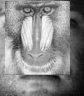
\includegraphics[\imagesizestring=.3\textwidth]{figures_iccv/yale_exp/1/y.png}}\\
\end{itemize}
\end{column}
\begin{column}{0.6\textwidth}
\renewcommand{\imagesizea}{0.15\textheight}
\begin{tabular}{cccc}
{\footnotesize Iteration} & {\footnotesize $\e$} & {\footnotesize $\s$} & {\footnotesize $Reconstruction$} \\
{\footnotesize 1} &
\fbox{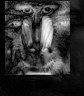
\includegraphics[\imagesizestring = \imagesizea]{figures_iccv/yale_exp/1/e.png}}&
\fbox{
\includegraphics[\imagesizestring = \imagesizea]{figures_iccv/yale_exp/1/L.png}}&
\fbox{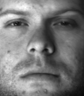
\includegraphics[\imagesizestring = \imagesizea]{figures_iccv/yale_exp/1/y_rec.png}}\\
{\footnotesize 2} &
\fbox{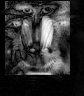
\includegraphics[\imagesizestring = \imagesizea]{figures_iccv/yale_exp/2/e.png}}&
\fbox{
\includegraphics[\imagesizestring = \imagesizea]{figures_iccv/yale_exp/2/L.png}}&
\fbox{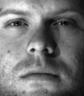
\includegraphics[\imagesizestring = \imagesizea]{figures_iccv/yale_exp/2/y_rec.png}}\\
{\footnotesize last} &
\fbox{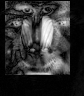
\includegraphics[\imagesizestring = \imagesizea]{figures_iccv/yale_exp/6/e.png}}&
\fbox{
\includegraphics[\imagesizestring = \imagesizea]{figures_iccv/yale_exp/6/L.png}}&
\fbox{\includegraphics[\imagesizestring = \imagesizea]{figures_iccv/yale_exp/6/y_rec.png}}
\end{tabular}
\end{column}
\end{columns}\renewcommand{\imagesizestring}{height}
}

\frame{\frametitle{Yale Results}
%\includegraphics[width=.5\textwidth]{figures_iccv/results/yale_lambda.pdf}\\
\begin{center}
\includegraphics[width=.5\textwidth]{figures_iccv/results/yale_cmp.pdf}\\
The MRF based algorithm (Algorithm 1) out-performs SRC (L1)
\end{center}
}

\renewcommand{\imagesizestring}{width}
\renewcommand{\imagesizea}{0.2\textwidth}
\frame{\frametitle{Natural Occlusion Example on AR Database}
\begin{columns}
\begin{column}{0.4\textwidth}
\begin{itemize}
\item Image from AR Database
\item Scarf occlusion
\item $\lambda = 3$
\item Test Image: \\
\fbox{\includegraphics[\imagesizestring=.3\textwidth]{figures_iccv/AR_exp/1/y.png}}
\end{itemize}
\end{column}
\begin{column}{0.6\textwidth}
\renewcommand{\imagesizea}{0.15\textheight}
\begin{tabular}{cccc}
{\footnotesize Iteration} & {\footnotesize $\e$} & {\footnotesize $\s$} & {\footnotesize $Reconstruction$} \\
{\footnotesize 1} &
\fbox{\includegraphics[\imagesizestring = \imagesizea]{figures_iccv/AR_exp/1/e.png}}&
\fbox{\includegraphics[\imagesizestring = \imagesizea]{figures_iccv/AR_exp/1/L.png}}&
\fbox{\includegraphics[\imagesizestring = \imagesizea]{figures_iccv/AR_exp/1/y_rec.png}}\\
{\footnotesize 2} &
\fbox{\includegraphics[\imagesizestring = \imagesizea]{figures_iccv/AR_exp/2/e.png}}&
\fbox{\includegraphics[\imagesizestring = \imagesizea]{figures_iccv/AR_exp/2/L.png}}&
\fbox{\includegraphics[\imagesizestring = \imagesizea]{figures_iccv/AR_exp/2/y_rec.png}}\\
{\footnotesize last} &
\fbox{\includegraphics[\imagesizestring = \imagesizea]{figures_iccv/AR_exp/7/e.png}}&
\fbox{\includegraphics[\imagesizestring = \imagesizea]{figures_iccv/AR_exp/7/L.png}}&
\fbox{\includegraphics[\imagesizestring = \imagesizea]{figures_iccv/AR_exp/7/y_rec.png}}\\
\end{tabular}
\end{column}
\end{columns}\renewcommand{\imagesizestring}{height}
}

\frame{\frametitle{Natural Occlusion Results on AR Database}
\renewcommand{\imagesizea}{0.30\textwidth}
\vspace{-.2in}
\begin{columns}
\begin{column}{.33\textwidth}
{\tiny AR Database, 100 subjects, 800 images per subject. 200 test images, full size is $83\times 60$ }\\
\vspace{.3in} \ \\
{\tiny Extended Yale B Database Training: 19 subjects, Testing: 19 of same, 19 of different subjects, $96\times 84$ pixels.  Applied threshold to $\min_k \frac{\| \y^* - A_k^* \hat{\x}_k \|_1}{  | \{ i \mid \s_k[i] = -1 \} |^2}$ } \\
%{\tiny 60\% occlusion} & {\tiny 80\% occlusion}\\
%{\tiny Scarf} & {\tiny Sunglasses}\\
\end{column}
\begin{column}{.33\textwidth}
\begin{center}
\includegraphics[width=.9\textwidth]{figures_iccv/results/AR_scarf_new.pdf}\\
\vspace{-.1in}{\tiny Scarf}
\includegraphics[width=.9\textwidth]{figures_iccv/roc/eYB-60.pdf}\\
\vspace{-.1in}{\tiny 60\% occlusion}
\end{center}
\end{column}
\begin{column}{.33\textwidth}
\begin{center}
\includegraphics[width= .9\textwidth]{figures_iccv/results/AR_sunglasses_new.pdf}\\
\vspace{-.1in}{\tiny Sunglasses}
\includegraphics[width=.9\textwidth]{figures_iccv/roc/eYB-80.pdf}\\
\vspace{-.1in}{\tiny 80\% occlusion}
\end{center}
\end{column}
\end{columns}

}

\frame{\frametitle{MRF vs. SRC on Our Dataset}
\newcommand{\imagewidth}{.55in}
\vspace{-.12in}
{\tiny Training: 116 subjects, 38 images each, aligned using algorithm in previous section initialized by hand.}\\
\vspace{-.2in}
\begin{center}
\begin{tabular}{cccccc}
& {\small Normal} & {\small Eyeglasses} & {\small Sunglasses} & {\small Hats} & {\small Disguises} \\ [-.05in]
{\tiny \# Testing Images} & {\tiny 354} & {\tiny 118} & {\tiny 126} & {\tiny 40} & {\tiny 217}\\
& \includegraphics[width=\imagewidth]{figures_iccv/real_data_examples/normal_1.jpg} & \includegraphics[width=\imagewidth]{figures_iccv/real_data_examples/glasses_1.jpg} & \includegraphics[width=\imagewidth]{figures_iccv/real_data_examples/sunglasses_1.jpg} & \includegraphics[width= \imagewidth]{figures_iccv/real_data_examples/hats_1.jpg} & \includegraphics[width=\imagewidth]{figures_iccv/real_data_examples/disguise_1.jpg} \\
& \includegraphics[width=\imagewidth]{figures_iccv/real_data_examples/normal_2.jpg} & \includegraphics[width=\imagewidth]{figures_iccv/real_data_examples/glasses_2.jpg} & \includegraphics[width=\imagewidth]{figures_iccv/real_data_examples/sunglasses_2.jpg} & \includegraphics[width=\imagewidth]{figures_iccv/real_data_examples/hats_2.jpg} & \includegraphics[width=\imagewidth]{figures_iccv/real_data_examples/disguise_2.jpg} \\
& \includegraphics[width=\imagewidth]{figures_iccv/real_data_examples/normal_3.jpg} & \includegraphics[width=\imagewidth]{figures_iccv/real_data_examples/glasses_3.jpg} & \includegraphics[width=\imagewidth]{figures_iccv/real_data_examples/sunglasses_3.jpg} & \includegraphics[width=\imagewidth]{figures_iccv/real_data_examples/hats_3.jpg} & \includegraphics[width=\imagewidth]{figures_iccv/real_data_examples/disguise_3.jpg} \\
{\small MRF Recognition} & 91.4\% & 90.9\% & {\bf 81.0\%} & {\bf 55.0\%} & {\bf 43.6\%}\\
{\small SRC Recognition} & {\bf 99.4}\% & {\bf 98.3}\% & 65.6\% & 40.0\% & 37.8\%
\end{tabular}
\end{center}
}
